\documentclass[letterpaper, 12pt]{report}
\usepackage[utf8]{inputenc}
\usepackage[english, spanish]{babel}
\usepackage{fullpage} % changes the margin
\usepackage{graphicx} 
\usepackage{enumitem} 
\usepackage{chngcntr}
\usepackage{setspace}
\counterwithin{figure}{section}
\renewcommand{\thesection}{\arabic{section}} 
\renewcommand{\thesubsection}{\thesection.\arabic{subsection}}
\renewcommand{\baselinestretch}{1.5}
\usepackage{float}
\usepackage{apacite}
\bibliographystyle{apacite}
\setlength\belowcaptionskip{10pt}
\linespread{1.5}

\begin{document}

\begin{titlepage}
	\centering
	
\includegraphics[width=0.3\textwidth]{Images/logo_utb.png}\par\vspace{1cm}
	{\scshape\LARGE Universidad Tecnológica de Bolívar \par}
	\vspace{1cm}

	{\scshape\Large FÍSICA ELÉCTRICA \par}
	\vspace{.2cm}

	% chktex-file 8
	{\scshape\Large H1 - C \par}
	\vspace{1cm}
	% chktex-file 8
	\slshape {\Large \bfseries{} LAB 2 - MEDICIÓN DE DIFERENCIA DE POTENCIAL, CORRIENTE Y RESISTENCIA \\}
	\vspace{1cm}

	\slshape {\itshape{} Mauro González, T00067622 \\}
	\slshape {\itshape{} German De Armas Castaño, T00068765 \\}
	\slshape {\itshape{} Angel Vega Rodriguez, T00068186 \\}
	\slshape {\itshape{} Juan Jose Osorio Ariza, T00067316 \\}
	\slshape {\itshape{} Juan Eduardo barón, T00065901 \\}
	\vfill
	Revisado Por \\
	Gabriel Hoyos Gomez Casseres\\
	{\large \today\par}
\end{titlepage}

% ----------------------------------------------------------------------|>
\section{Introducción}

En esta segunda practica de laboratorio se usaran herramientas como la 
fuente de corriente directa, resistencias y multímetros para medir ciertos 
elementos y su flujo de corriente eléctrica con su respectiva diferencia 
de potencial. 

\vspace{.5cm}

Esta sesión tiene como objetivo enseñar el debido procedimiento
para usar diversos instrumentos, la familiarización de ciertos conceptos 
e incluso de unidades de medida.

\newpage

% ----------------------------------------------------------------------|>
\section{Objetivos}

\subsection{Objetivo General}

Aprender a utilizar todos los elementos con que cuenta el panel de las 
fuentes, asi como medir diferencia de potencial,corriente y resistencia 
tanto de un multímetro digital como analógico.

% ----------------------------------------------------------------------|>
\section{Preparación de la practica}

% -------------------------------------|>
\subsection{¿Qué es corriente y cuál es su unidad de medida? ¿Qué significa
	una corriente de 1A?}

R// La corriente es la velocidad a la que un flujo de electrones pasa por un
punto de un circuito eléctrico completo. Del modo más básico,
la corriente es igual al flujo.~\cite{DefinicionCorrientePlusAmperio}

\vspace{.5cm}

Un amperio (AM-pir) o A es la unidad internacional para la medición de la
corriente. Expresa la cantidad de electrones
(a veces llamada ``carga eléctrica``) que pasan por punto en un circuito
durante un tiempo determinado.~\cite{DefinicionCorrientePlusAmperio}

\vspace{.5cm}

Esto quiere decir, que para referirnos a ``¿Cuanta corriente pasa por un
punto en un circuito?``, se utilizan los amperios, es decir, una carga de 1A
significa que 1 Culombio de electrones pasa por ese punto en el circuito en
1 segundo.~\cite{DefinicionCorrientePlusAmperio}

% -------------------------------------|>
\subsection{¿Qué es resistencia y cuál es su unidad de medida? ¿Qué
	significa una resistencia de 1Ω?}

R// La resistencia es una medida de la oposición del flujo de corriente.
~\cite{DefinicionResistenciaPlusOhmios}

\vspace{.5cm}

La resistencia se mide en ohmios, que se simbolizan con la letra griega
omega (Ω). Se denominaron ohmios en honor a Georg Simon Ohm (1784 a 1854),
un físico alemán que estudió la relación entre voltaje, corriente y
resistencia. Se le atribuye la formulación de la ley de Ohm.
~\cite{DefinicionResistenciaPlusOhmios}

\vspace{.5cm}

Tomando como referencia un valor de resistencia de 1Ω, cuanto mayor sea este
numero, menor será el flujo de corriente; Asimismo cuanto menor sea la
resistencia, mayor será el flujo de la corriente.
~\cite{DefinicionResistenciaPlusOhmios}

% -------------------------------------|>
\subsection{¿Cómo se determina una resistencia por su código de
	colores? Muestre un ejemplo.}

R// El código de colores se utiliza en electrónica para indicar los
valores de los componentes electrónicos. Es muy habitual en los resistores
pero también se utiliza para otros componentes como condensadores,
inductores, diodos etc.~\cite{CodigoColores}

\vspace{.5cm}

Las dos primeras franjas desde la izquierda, indican las primeras cifras
del valor del componente, mientras que una tercera indica por cuanto debe
multiplicarse el valor de la cifra leída. La última franja, más separada
del resto, y típicamente de color dorado o plata, indica la tolerancia,
es decir, el margen de error que garantiza el fabricante. En el caso de
las resistencias de precisión, se cuenta con seis bandas de colores: las
tres primeras indican cifras, la cuarta el multiplicador, la quinta la
tolerancia y la sexta, el coeficiente de temperatura. El resto de franjas
indica la mantisa (cifras significativas) y el exponente del valor
nominal. De esta manera, una resistencia de las series E12 o E24, que
están normalizadas con 2 cifras significativas, llevan cuatro franjas: las
dos cifras, el exponente o factor potencia de 10, y la tolerancia.

\vspace{.5cm}

\begin{figure}[H]
	\begin{center}
		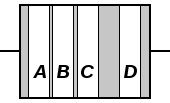
\includegraphics[scale = .8]{./Images/BandasResistores.svg}
		\caption{Diagrama de una resistencia}
	\end{center}
\end{figure}

\begin{figure}[H]
	\begin{center}
		
\includegraphics[scale = .8]{./Images/RepresentacionBandasResistores.svg}
		\caption{Diagrama de código de colores}
	\end{center}
\end{figure}

\begin{figure}[H]
	\centering

	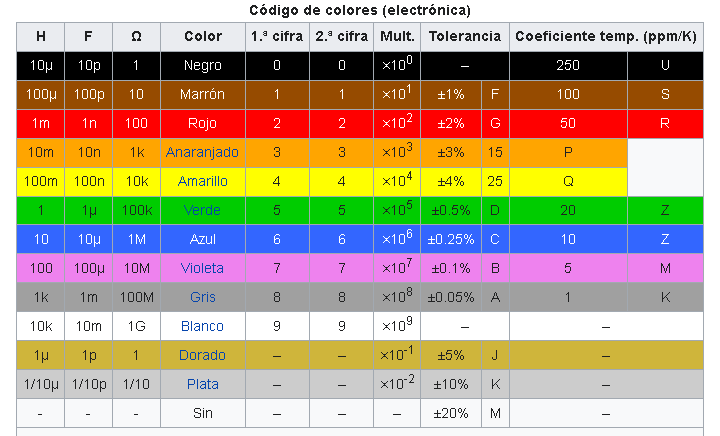
\includegraphics[scale = .65]{./Images/TablaDeColoresResistencias}

	\caption{Tabla de colores de las resistencias}
	\label{Tabla de colores de las resistencias}
\end{figure}

Según la tabla~\ref{Tabla de colores de las resistencias}, si tenemos
respectivamente una resistencia con los colores Amarillo, Verde, Rojo,
Anaranjado, esto quiere decir que el valor de la resistencia sera igual a
45 $\times{}$ $10^2$ $\pm$ $10^3$ Ω (Ohmios).

% -------------------------------------|>
\subsection{¿Cómo se conecta a un circuito un amperímetro,
	un voltímetro? ¿cómo se utiliza un ohmímetro?}

\begin{itemize}
	\item Amperímetro \hfill \break{}
	      El amperímetro se coloca intercalado en el circuito en el que queremos
	      medir la intensidad de corriente (circulación de electrones): es como
	      cortar el cable en un punto e intercalar entre los dos extremos del
	      cable el amperímetro. Esto es lo que se llama colocarlo en serie
	      con el circuito.

	      Al colocarlo así, toda la corriente del circuito circula por el
	      amperímetro. El circuito tiene ahora una resistencia añadida (RA)
	      porque el amperímetro lo ``carga' y ya no es el circuito que queríamos
	      estudiar, sino uno modificado.

	      Para minimizar este efecto ponemos, paralelo al ``mecanismo' del
	      amperímetro y dentro de él, un cable ``grueso' (con poca resistencia)
	      para que casi toda la corriente pase por el cable y sólo una parte
	      vaya al mecanismo del amperímetro.~\cite{Amperimetro}

	\item Voltímetro \hfill \break{}
	      Un voltímetro mide la diferencia en voltaje entre dos puntos de un
	      circuito eléctrico y por lo tanto, se debe conectar en paralelo con
	      la porción del circuito sobre el que se quiere realizar
	      la medida.~\cite{Voltimetro}

	\item Ohmímetro \hfill \break{}
	      La resistencia se mide con un ohmímetro, y se conecta entre los dos
	      extremos de la resistencia a medir, estando ésta desconectada
	      del circuito eléctrico.~\cite{Ohmimetro}
\end{itemize}

% -------------------------------------|>
\subsection{¿Qué es una fuente de corriente directa?}

R// La corriente directa (CD) o corriente continua (CC) es aquella cuyas
cargas eléctricas o electrones fluyen siempre en el mismo sentido en un
circuito eléctrico cerrado, moviéndose del polo negativo hacia el polo
positivo de una fuente de fuerza electromotriz (FEM).

\vspace{.5cm}

En otras palabras, la corriente directa es un flujo eléctrico que se mantiene
constante y no hay cambios en el voltaje.~\cite{CorrienteContinua}

% -------------------------------------|>
\subsection{¿Qué es una fuente de corriente alterna? ¿Qué es el voltaje RMS?}

R// La corriente alterna (CA) es un tipo de corriente eléctrica, en
la que la dirección del flujo de electrones va y viene a intervalos
regulares o en ciclos. La corriente que fluye por las líneas eléctricas
y la electricidad disponible normalmente en las casas procedente de los
enchufes de la pared es corriente alterna.~\cite{CorrienteAlterna}

\vspace{.5cm}

El voltaje RMS, o el cuadrado medio de la raíz
(también llamado el voltaje eficaz), es un método de denotar una forma de
onda senoidal de voltaje (forma de onda de CA) como un voltaje equivalente
que representa el valor de voltaje DC que producirá el mismo efecto de
calentamiento o disipación de potencia en el circuito,
como esta tensión de CA.\@~\cite{VoltajeRMS}

\vspace{.5cm}

En otras palabras, la forma de onda es una forma de onda AC, pero el
valor RMS permite que esta forma de onda se especifique como DC, porque
es la tensión DC equivalente que entrega la misma cantidad de energía a
una carga en un circuito como la señal AC hace sobre
su ciclo.~\cite{VoltajeRMS}

% -------------------------------------|>
\subsection{¿Cuál es la relación entre corriente, resistencia
	y voltaje en un circuito (Ley de Ohm)?}

R// La ley de Ohm se usa para determinar la relación entre tensión,
corriente y resistencia en un circuito eléctrico.~\cite{LeyDeOhm}

\vspace{.5cm}

Cuando se enuncia en forma explícita, significa que tensión es igual a la
corriente por la resistencia.~\cite{LeyDeOhm}

\vspace{.7cm}

La ley de Ohm recibió su nombre en honor al físico alemán Georg Ohm
(1789 a 1854) y aborda las cantidades clave en funcionamiento en
los circuitos.~\cite{LeyDeOhm}

% ----------------------------------------------------------------------|>
\section{Resumen del procedimiento}

En este experimento vamos a utilizar multímetro digital y un multímetro 
análogo conectado mediante cables a un panel de fuentes. Después procedemos 
a medir la resistencia, voltaje y corriente eléctrica. Y anotarlos los 
resultados que nos muestra los multímetros, Y por último repetimos las 
mediciones  cambiando los valores para poder comparar los datos entre los 
dos tipos de multímetros.

\newpage
\bibliography{./Bibliography/bibliography.bib}

\end{document}